\documentclass[border=5pt]{standalone}
\usepackage{tikz}
\usetikzlibrary{arrows.meta,positioning,shapes.geometric,fit,calc,decorations.pathreplacing,backgrounds}
\usepackage{xcolor}
\usepackage{amsmath}
\usepackage{booktabs}

% Color palette
\definecolor{arxivred}{HTML}{B31B1B}
\definecolor{goldmedal}{HTML}{FFD700}
\definecolor{silvermedal}{HTML}{C0C0C0}
\definecolor{bronzemedal}{HTML}{CD7F32}
\definecolor{advisorblue}{HTML}{2563EB}
\definecolor{engineergreen}{HTML}{16A34A}
\definecolor{thinkerorg}{HTML}{EA580C}
\definecolor{researchpurp}{HTML}{7C3AED}
\definecolor{analystcyan}{HTML}{0891B2}

\begin{document}

% ===== FIGURE 1: Hero figure — From Papers to Medals Pipeline =====
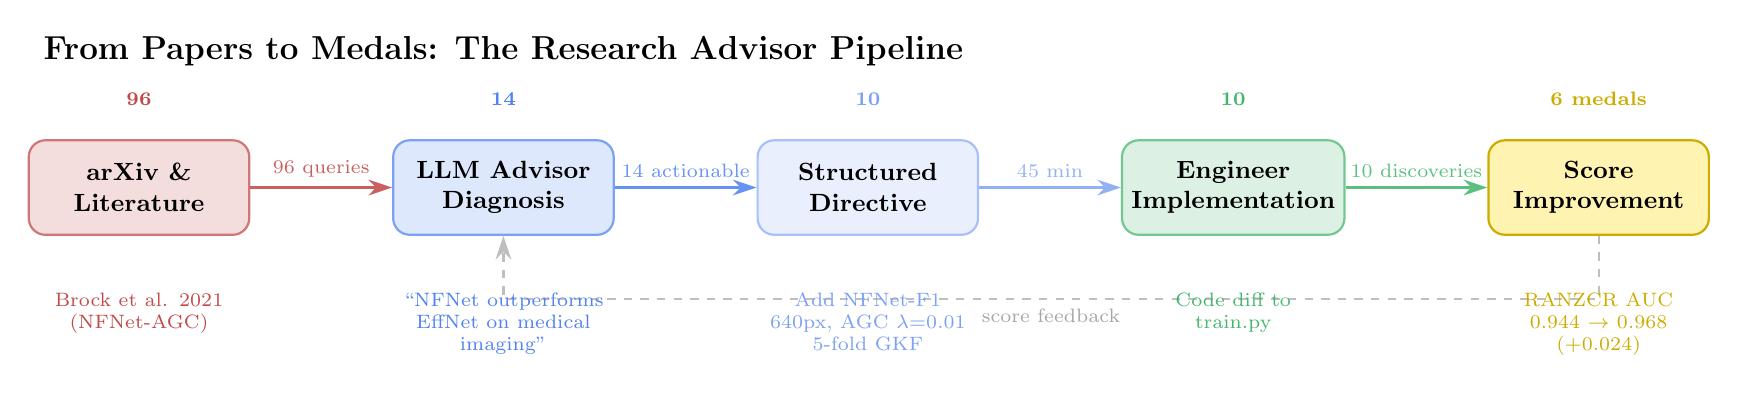
\begin{tikzpicture}[
    stage/.style={draw, rounded corners=6pt, minimum width=2.8cm, minimum height=1.2cm, font=\small\bfseries, align=center, thick},
    arrow/.style={-{Stealth[length=3mm,width=2mm]}, thick, #1},
    arrow/.default={black},
    note/.style={font=\scriptsize, text width=2.5cm, align=center},
    every node/.style={font=\small}
]

% Stage 1: Literature
\node[stage, fill=arxivred!15, draw=arxivred!60] (lit) {arXiv \&\\Literature};

% Stage 2: Advisor Diagnosis
\node[stage, fill=advisorblue!15, draw=advisorblue!60, right=1.8cm of lit] (diag) {LLM Advisor\\Diagnosis};

% Stage 3: Directive
\node[stage, fill=advisorblue!10, draw=advisorblue!40, right=1.8cm of diag] (dir) {Structured\\Directive};

% Stage 4: Implementation
\node[stage, fill=engineergreen!15, draw=engineergreen!60, right=1.8cm of dir] (impl) {Engineer\\Implementation};

% Stage 5: Result
\node[stage, fill=goldmedal!30, draw=goldmedal!80!black, right=1.8cm of impl] (result) {Score\\Improvement};

% Arrows between stages
\draw[arrow=arxivred!70] (lit) -- (diag) node[midway, above, font=\scriptsize] {96 queries};
\draw[arrow=advisorblue!70] (diag) -- (dir) node[midway, above, font=\scriptsize] {14 actionable};
\draw[arrow=advisorblue!50] (dir) -- (impl) node[midway, above, font=\scriptsize] {45 min};
\draw[arrow=engineergreen!70] (impl) -- (result) node[midway, above, font=\scriptsize] {10 discoveries};

% Feedback loop
\draw[arrow=gray!50, dashed] (result.south) -- ++(0,-0.8) -| (diag.south) node[pos=0.25, below, font=\scriptsize, text=gray!70] {score feedback};

% Example annotations below
\node[below=0.6cm of lit, font=\scriptsize, text=arxivred!80, text width=2.5cm, align=center] {Brock et al. 2021\\(NFNet-AGC)};
\node[below=0.6cm of diag, font=\scriptsize, text=advisorblue!80, text width=3cm, align=center] {``NFNet outperforms\\EffNet on medical\\imaging''};
\node[below=0.6cm of dir, font=\scriptsize, text=advisorblue!60, text width=2.8cm, align=center] {Add NFNet-F1\\640px, AGC $\lambda$=0.01\\5-fold GKF};
\node[below=0.6cm of impl, font=\scriptsize, text=engineergreen!80, text width=2.5cm, align=center] {Code diff to\\train.py};
\node[below=0.6cm of result, font=\scriptsize, text=goldmedal!80!black, text width=2.5cm, align=center] {RANZCR AUC\\0.944 $\rightarrow$ 0.968\\(+0.024)};

% Title
\node[above=0.8cm of diag, anchor=south, font=\large\bfseries] {From Papers to Medals: The Research Advisor Pipeline};

% Funnel numbers at top
\node[above=0.3cm of lit, font=\scriptsize\bfseries, text=arxivred!80] {96};
\node[above=0.3cm of diag, font=\scriptsize\bfseries, text=advisorblue!80] {14};
\node[above=0.3cm of dir, font=\scriptsize\bfseries, text=advisorblue!60] {10};
\node[above=0.3cm of impl, font=\scriptsize\bfseries, text=engineergreen!80] {10};
\node[above=0.3cm of result, font=\scriptsize\bfseries, text=goldmedal!80!black] {6 medals};

\end{tikzpicture}

\end{document}
